% Segmentation Pipeline section. Paste into your own thesis, or \input it.

\section{Evaluation metrics}
\label{sec:pipeline-metrics}

Evaluation reads the saved predictions and the matching GT masks and centerlines, and scores one
against the other. The GT mask, a full 3D volume label, is what Dice, HD95 and the Betti numbers
below are scored against. The GT centerline is what the centerline metrics below are scored
against; it is a precomputed file, not something this pipeline derives, and it is itself a
skeleton of the corrected GT lumen mask, produced during dataset curation and then Gaussian
smoothed and manually reviewed for its segment labels \cite{bransby2026imagecasx}. The predicted
centerline has no such curated file to draw on, so it is instead skeletonised from the predicted
mask directly at evaluation time, with none of that smoothing or review. No single number fully
captures
what a good segmentation of a thin, branching
structure means, so the benchmark reports several metric families together
\cite{taha2015metrics}, each computed at the scan's original resolution so distances and volumes
are in true physical units (\texttt{utils/metrics.py}).

\textbf{Dice} (Equation~\ref{eq:pipeline-dice}) answers how much of the vessel, by volume, was
found. It is normalised by $|P|+|G|$, the size of the two regions being compared, not by the
scan's total voxel count, so it stays meaningful for a structure this small: an empty prediction
scores 0, not the 99\,\%+ that whole-volume accuracy would give it for correctly ignoring the
background (top of Figure~\ref{fig:pipeline-dice-hd95}). \textbf{HD95} complements Dice as a
worst-case, boundary-based measure instead of a volume-averaged one:
\[
  \mathrm{HD95}(P,G) = \max\Big(P_{95}\big(d_{G\to P}\big),\ P_{95}\big(d_{P\to G}\big)\Big),
\]
where $d_{G\to P}$ is the set of distances from every voxel on the GT surface to the nearest
predicted voxel ($d_{P\to G}$ the same in reverse), and $P_{95}$ is the 95th percentile. Taking
the worst of the two directions, rather than pooling them, means a boundary that is well matched
one way but poorly matched the other cannot average the error away; the 95th percentile rather
than the true maximum discards only the single most extreme outlier voxel, which keeps one bad
voxel from dominating the whole score. Figure~\ref{fig:pipeline-dice-hd95} shows both metrics in
turn.

\begin{figure}[htbp]
  \centering
  \begin{tikzpicture}[font=\sffamily\small]
    \draw[draw=black!50, fill=black!6] (0,0) rectangle (2.6,2.6);
    \node[font=\sffamily\footnotesize, align=center] at (1.3,2.9)
      {full scan volume\\(e.g.\ $400^3$ voxels)};

    \coordinate (spot) at (1.75,0.7);
    \draw[draw=blue!60!black, fill=orange!40!blue!20] (spot) circle (2pt);

    \node[font=\sffamily\scriptsize, align=center, text width=2.1cm] at (0.75,0.35)
      {background:\\never enters Dice};
    \draw[-{Latex[length=1.1mm]}, black!50] (1.15,0.5) -- (1.65,0.67);

    \coordinate (zC) at (4.9,1.3);
    \def\zR{1.05}
    \draw[dashed, black!40] (spot) -- ($(zC)+(-\zR,\zR)$);
    \draw[dashed, black!40] (spot) -- ($(zC)+(-\zR,-\zR)$);

    \begin{scope}[shift={(zC)}]
      \draw[draw=black!40, fill=white] (0,0) circle (\zR);
      \begin{scope}
        \clip (0,0) circle (\zR);
        \draw[draw=blue!60!black, fill=blue!12] (-0.27,0) circle (0.74);
        \draw[draw=orange!80!black, fill=orange!15] (0.27,0) circle (0.62);
        \begin{scope}
          \clip (-0.27,0) circle (0.74);
          \fill[green!45!black, opacity=0.4] (0.27,0) circle (0.62);
        \end{scope}
      \end{scope}
      \draw[draw=black!40] (0,0) circle (\zR);
      \node[font=\sffamily\scriptsize] at (-0.78,0.12) {GT};
      \node[font=\sffamily\scriptsize] at (0.8,0.12) {Pred};
      \node[font=\sffamily\tiny] at (0,0) {$P\cap G$};
      \node[below, font=\sffamily\footnotesize, align=center] at (0,-1.3)
        {\textbf{Dice} $= \dfrac{2\,|P\cap G|}{|P|+|G|}$};
    \end{scope}

    \begin{scope}[xshift=8.2cm, yshift=1.3cm]
      \def\gtR{1.35}
      \def\predCx{1.0}
      \def\predR{1.1}
      \draw[draw=blue!60!black] (0,0) circle (\gtR);
      \draw[draw=orange!80!black] (\predCx,0) circle (\predR);
      \foreach \ang [count=\i] in {100, 150, 180, 210, 260} {
        \pgfmathsetmacro{\gx}{\gtR*cos(\ang)}
        \pgfmathsetmacro{\gy}{\gtR*sin(\ang)}
        \pgfmathsetmacro{\dx}{\gx-\predCx}
        \pgfmathsetmacro{\dy}{\gy}
        \pgfmathsetmacro{\norm}{sqrt(\dx*\dx+\dy*\dy)}
        \pgfmathsetmacro{\tx}{\predCx+\predR*\dx/\norm}
        \pgfmathsetmacro{\ty}{\predR*\dy/\norm}
        \ifnum\i=3
          \draw[-{Latex[length=1.7mm]}, red!70!black, very thick] (\gx,\gy) -- (\tx,\ty);
        \else
          \draw[-{Latex[length=1.2mm]}, black!50, thin] (\gx,\gy) -- (\tx,\ty);
        \fi
      }
      \node[font=\sffamily\footnotesize] at (-0.75,1.1) {GT};
      \node[font=\sffamily\footnotesize] at (2.0,0.85) {Pred};
      \node[below, font=\sffamily\footnotesize, align=center] at (0.5,-1.6)
        {$d_{G\to P}$: GT surface\\to nearest Pred point};
    \end{scope}
  \end{tikzpicture}
  \caption{\emph{Left}: Dice is computed relative to the vessel's own extent, not the scan's: the
    dot marks how small the true lumen (well under 1\% of the volume) is against the full scan,
    magnified alongside. \emph{Right}: HD95 scores the boundary instead: thin arrows are sample
    GT-surface points paired with their nearest Pred-surface point, and the red arrow is the
    farthest of these sample distances, standing in for the 95th-percentile value this direction
    contributes. The reverse direction, Pred surface to nearest GT point, is computed the same
    way and not shown; HD95 takes the worse of the two, so a boundary matched well in only one
    direction cannot hide behind the other.}
  \label{fig:pipeline-dice-hd95}
\end{figure}

\textbf{Betti numbers} count topological errors that Dice and HD95 are largely blind to: $\beta_0$
is the number of separate connected components and $\beta_1$ the number of loops, the only two
the benchmark scores. $\beta_1$ is derived from the mask's Euler characteristic $\chi$
(\texttt{skimage.measure.euler\_number}) via
\[
  \beta_1 = \max(0,\ \beta_0 - \chi),
\]
which gives the exactly correct count for a tube-shaped structure like a vessel tree, since a tube
never has a sealed pocket of empty space trapped inside it. The benchmark reports the absolute
error in each against the GT, so a mask that is broken into
fragments or contains a spurious loop between two branches is penalised even if its overlap and
boundary distance both look fine (Figure~\ref{fig:pipeline-betti}).

\begin{figure}[htbp]
  \centering
  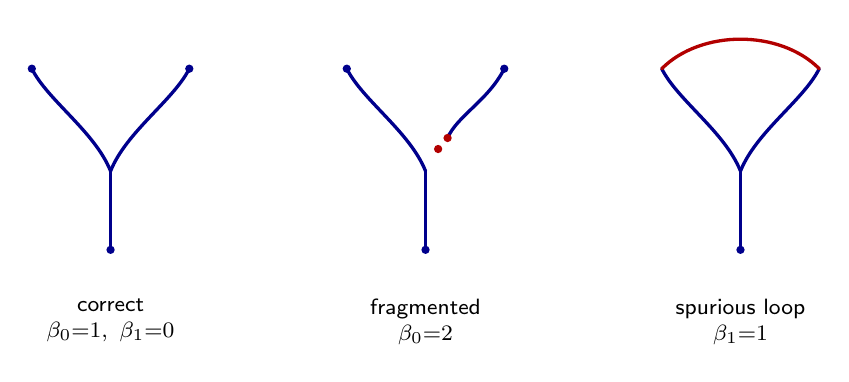
\begin{tikzpicture}[font=\sffamily\small,
      tube/.style={very thick, blue!55!black, line cap=round},
      tip/.style={circle, fill=blue!55!black, inner sep=0pt, minimum size=3pt}]
    \begin{scope}
      \draw[tube] (0,-1) -- (0,0);
      \draw[tube] (0,0) .. controls (-0.2,0.5) and (-0.8,0.9) .. (-1,1.3);
      \draw[tube] (0,0) .. controls (0.2,0.5) and (0.8,0.9) .. (1,1.3);
      \node[tip] at (0,-1) {};
      \node[tip] at (-1,1.3) {};
      \node[tip] at (1,1.3) {};
      \node[below, align=center, font=\sffamily\footnotesize] at (0,-1.5)
        {correct\\$\beta_0{=}1,\ \beta_1{=}0$};
    \end{scope}
    \begin{scope}[xshift=4cm]
      \draw[tube] (0,-1) -- (0,0);
      \draw[tube] (0,0) .. controls (-0.2,0.5) and (-0.8,0.9) .. (-1,1.3);
      \draw[tube] (0.28,0.42) .. controls (0.4,0.7) and (0.8,0.9) .. (1,1.3);
      \node[tip] at (0,-1) {};
      \node[tip] at (-1,1.3) {};
      \node[tip] at (1,1.3) {};
      \node[tip, fill=red!70!black] at (0.28,0.42) {};
      \node[tip, fill=red!70!black] at (0.16,0.28) {};
      \node[below, align=center, font=\sffamily\footnotesize] at (0,-1.5)
        {fragmented\\$\beta_0{=}2$};
    \end{scope}
    \begin{scope}[xshift=8cm]
      \draw[tube] (0,-1) -- (0,0);
      \draw[tube] (0,0) .. controls (-0.2,0.5) and (-0.8,0.9) .. (-1,1.3);
      \draw[tube] (0,0) .. controls (0.2,0.5) and (0.8,0.9) .. (1,1.3);
      \draw[tube, red!70!black] (-1,1.3) .. controls (-0.5,1.8) and (0.5,1.8) .. (1,1.3);
      \node[tip] at (0,-1) {};
      \node[below, align=center, font=\sffamily\footnotesize] at (0,-1.5)
        {spurious loop\\$\beta_1{=}1$};
    \end{scope}
  \end{tikzpicture}
  \caption{Three predictions of the same branching vessel, schematically. Left: correct topology,
    one component and no loops. Middle: a break partway along a branch (red dots) splits it into a
    second, disconnected component, penalised even though the missing segment is a single thin
    stretch. Right: an erroneous extra connection between the two branch tips closes a cycle that
    is not anatomically real. Dice and HD95 would barely register either error; Betti numbers are
    built to catch exactly this kind of mistake.}
  \label{fig:pipeline-betti}
\end{figure}

Three further metrics target the vessel's 1D \textbf{centerline} rather than its full volume.
\textbf{clDice} \cite{shit2021cldice} applies Dice's own harmonic-mean form, but between each
mask's skeleton and the \emph{other} mask's full volume:
\[
  \mathrm{clDice} = \frac{2\,T_{\mathrm{prec}}\,T_{\mathrm{sens}}}{T_{\mathrm{prec}}+T_{\mathrm{sens}}},
  \qquad T_{\mathrm{prec}} = \frac{|S_P \cap G|}{|S_P|}, \quad
  T_{\mathrm{sens}} = \frac{|S_G \cap P|}{|S_G|},
\]
for predicted and GT skeletons $S_P, S_G$. Because a thin skeleton has almost no volume of its own
to fall back on, a single connectivity-breaking gap removes a large share of $S_P$ or $S_G$ from
the other mask, making clDice far more sensitive to exactly that failure than whole-volume Dice
is. \textbf{Centerline mean distance} and \textbf{centerline HD95} instead compare the predicted
skeleton directly against the GT's separately annotated centerline points, the same mean/95th-percentile
logic as Dice/HD95 applied to 1D point sets rather than 3D surfaces. Predicted and GT lumen volumes
are also reported directly, alongside their absolute and signed difference.

Beyond one number per scan, every metric is also broken down by scan-level subgroup (image
quality, dominance, disease status) and by location along the vessel: a local Dice computed in an
8\,mm cube around points sampled along the GT centerline, grouped by coronary segment, distance
from the ostium, local diameter and local HU attenuation, so a result can be read as, for
instance, holding up proximally but degrading distally, tracking the vessel's shrinking diameter.
